%---------------------------------------------------------------------------%
%-                                                                         -%
%-                           LaTeX Template                                -%
%-                                                                         -%
%---------------------------------------------------------------------------%
%- Copyright (C) Huangrui Mo <huangrui.mo@gmail.com> 
%- This is free software: you can redistribute it and/or modify it
%- under the terms of the GNU General Public License as published by
%- the Free Software Foundation, either version 3 of the License, or
%- (at your option) any later version.
%---------------------------------------------------------------------------%
%->> Document class declaration
%---------------------------------------------------------------------------%
\documentclass[oneside]{Style/ucasthesis}%
%- Multiple optional arguments:
%- [<oneside|twoside|print>]% oneside eprint, twoside eprint, or paper print
%- [fontset=<adobe|none|...>]% specify font set instead of automatic detection
%- [scheme=plain]% thesis writing of international students
%- [draftversion]% show draft version information
%- [standard options for ctex book class: draft|paper size|font size|...]%
%---------------------------------------------------------------------------%
%->> Document settings
%---------------------------------------------------------------------------%
\usepackage[authoryear,list]{Style/artratex}% document settings
%- usage: \usepackage[option1,option2,...,optionN]{artratex}
%- Multiple optional arguments:
%- [bibtex|biber]% set bibliography processor and package
%- [<numbers|super|authoryear|alpha>]% set citation and reference style
%- <numbers>: textual: Jones [1]; parenthetical: [1]
%- <super>: textual: Jones superscript [1]; parenthetical: superscript [1]
%- <authoryear>: textual: Jones (1995); parenthetical: (Jones, 1995)
%- <alpha>: textual: not available; parenthetical: [Jon95]
%- [geometry]% reconfigure page layout via geometry package
%- [lscape]% provide landscape layout environment
%- [xhf]% disable header and footer via fancyhdr package
%- [color]% provide color support via xcolor package
%- [background]% enable page background
%- [tikz]% provide complex diagrams via tikz package
%- [table]% provide complex tables via ctable package
%- [list]% provide enhanced list environments for algorithm and coding
%- [math]% enable some extra math packages
%- [xlink]% disable link colors
\usepackage{Style/artracom}% user defined commands
%---------------------------------------------------------------------------%
%->> Document inclusion
%---------------------------------------------------------------------------%
%\includeonly{Tex/Chap_1,...,Tex/Chap_N}% selected files compilation
%---------------------------------------------------------------------------%
%->> Document content
%---------------------------------------------------------------------------%
%-
%-> Titlepage information
%-
%---------------------------------------------------------------------------%
%->> Titlepage information
%---------------------------------------------------------------------------%
%-
%-> 中文封面信息
%-
\confidential{}% 密级:只有涉密论文才填写
\schoollogo[scale=0.095]{ucas_logo}% 校徽
\title{第X小组}% 论文中文题目
\author{XXX}% 论文作者
\advisor{\ XXX\ XXX\ XXX\ XXX\ \ }% 指导教师:姓名 专业技术职务 工作单位

\date{2020~年~12~月}% 毕业日期:夏季为6月、冬季为12月
%-
%-> 英文封面信息
%-
\DEGREE{Master}% 学位:Bachelor, Master, Doctor, Postdoctor。封面据英文学位名称自动切换,需确保拼写准确
%---------------------------------------------------------------------------%
%
%the external package we \usepackage 
\usepackage{booktabs}

\begin{document}
%-
%-> Frontmatter: title page, abstract, content list, symbol list, preface
%-
\frontmatter% initialize the environment
%---------------------------------------------------------------------------%
%->> Frontmatter
%---------------------------------------------------------------------------%
%-
%-> 生成封面
%-
\maketitle% 生成中文封面
%\MAKETITLE% 生成英文封面
%-
%-> 作者声明
%-
% \makedeclaration% 生成声明页
% %-
% %-> 中文摘要
% %-
% \intobmk\chapter*{摘\quad 要}% 显示在书签但不显示在目录
% \setcounter{page}{1}% 开始页码
% \pagenumbering{Roman}% 页码符号
% 本文是中国科学院大学学位论文模板ucasthesis的使用说明文档。主要内容为介绍\LaTeX{}文档类ucasthesis的用法,以及如何使用\LaTeX{}快速高效地撰写学位论文。
% \keywords{中国科学院大学,学位论文,\LaTeX{}模板}% 中文关键词
% %-
% %-> 英文摘要
% %-
% \intobmk\chapter*{Abstract}% 显示在书签但不显示在目录
% This paper is a help documentation for the \LaTeX{} class ucasthesis, which is  a thesis template for the University of Chinese Academy of Sciences. The main content is about how to use the ucasthesis, as well as how to write thesis efficiently by using \LaTeX{}.
% \KEYWORDS{University of Chinese Academy of Sciences (UCAS), Thesis, \LaTeX{} Template}% 英文关键词
% %---------------------------------------------------------------------------%% title page, abstract
% {% content list region
% \linespread{1.2}% local line space
% \intobmk*{\cleardoublepage}{\contentsname}% add link to bookmark
% \tableofcontents% content catalog
% \intobmk*{\cleardoublepage}{\listfigurename}% add link to bookmark
% \listoffigures% figure catalog
% \intobmk*{\cleardoublepage}{\listtablename}% add link to bookmark
% \listoftables% table catalog
% }
%\input{Tex/Prematter}% symbol list, preface content
%-
%-> Mainmatter
%-
\mainmatter% initialize the environment
%---------------------------------------------------------------------------%
%->> Main content
%---------------------------------------------------------------------------%
% \input{Tex/Chap_Intro}
% \input{Tex/Chap_Guide}
\chapter{关于本报告的说明}\label{chap:dscpt}

本报告是针对是提出神经网络经典模型AlexNet2012的论文《ImageNet Classification with Deep Convolutional Neural Networks》进行的写作规范研究报告。
\section{组织架构}

本报告的主体部分为第2-5章。

其中主体的第一部分是第~\ref{chap:other}章,分析的是该文章的标题、署名、摘要和引证等,并对摘要的结构和内容提出了一些值得商榷的意见。

本报告的主体第二部分是第~\ref{chap:introduction}章、第~\ref{chap:res}章,分析的是该文章的主体结构,其中第~\ref{chap:introduction}章是对文章引言的具体分析,第~\ref{chap:res}章是对文章方法、结果和讨论部分的具体分析。

本报告的主体第三部分是第~\ref{chap:figtbl}章,分析该文章中的图表风格特点,并提出了一些改进意见。

本报告的头尾两小章是对本报告的说明和小结。
\section{成员分工}
本小组的成员分工如下表所示:

% Table generated by Excel2LaTeX from sheet 'Sheet1'
\begin{table}[!htbp]
  \centering
  \caption{小组成员分工}
    \begin{tabular}{lll}
    \toprule
    \textbf{成员分工} & \multicolumn{1}{c}{\textbf{负责的部分}} & \multicolumn{1}{l}{\textbf{对应的正文内容}} \\
    \midrule
        XXX & 分析文章中的方法、结果和讨论 & 第~\ref{chap:res}章\\
        XXX & 分析文章中的图表 & 第~\ref{chap:figtbl}章\\
        XXX & 分析文章的引言 & 第~\ref{chap:introduction}章\\
        XXX & 分析论文的标题、署名、摘要、引证 & 第~\ref{chap:other}章\\
        XXX & 整合、报告排版 & 头尾两小章\\
    \midrule
    \end{tabular}%
  \label{tab:division}%
\end{table}%


\chapter{标题、摘要、引证、署名}\label{chap:other}
\section{标题}
文章的标题(如图~\ref{fig:title})简洁有力,以一句话文摘的形式反映了该文章研究的任务以及采用的方法这两项文章的精髓。标题的内容非常具体、准确、简练,均由术语构成,每个词都有明确的含义。在用词上,均采用名词短语,语法规范。

\begin{figure}[!htbp]
	\centering
	
\includegraphics[width=\textwidth]{title}
	\caption{文章的标题}
	\label{fig:title}
\end{figure}

\section{署名}
在署名的设计(如图~\ref{fig:signature})上,作者名称、单位以及邮箱采用不同的字体字号进行区分,并且排版工整,使得读者对于作者的信息一目了然。在署名的顺序上,可以看出,并不是按严格按名称首字母进行的排序,经过对作者的背景的研究,发现前两位作者是最后一位作者Hinton的学生,则署名顺序是以学生-导师的顺序完成,学生部分的署名按名称首字母的顺序排列。需要说明的是,由于该文章的三位作者都是深度学习领域公认的明星学者,因此该文章或许不存在所谓需要特别突出的“第一作者”。
\begin{figure}[!htbp]
	\centering
	
\includegraphics[width=\textwidth]{signature}
	\caption{文章的署名}
	\label{fig:signature}
\end{figure}

\section{摘要}
文章摘要的结构分析结果如图~\ref{fig:abstract}所示。

\begin{figure}[!htbp]
	\centering
	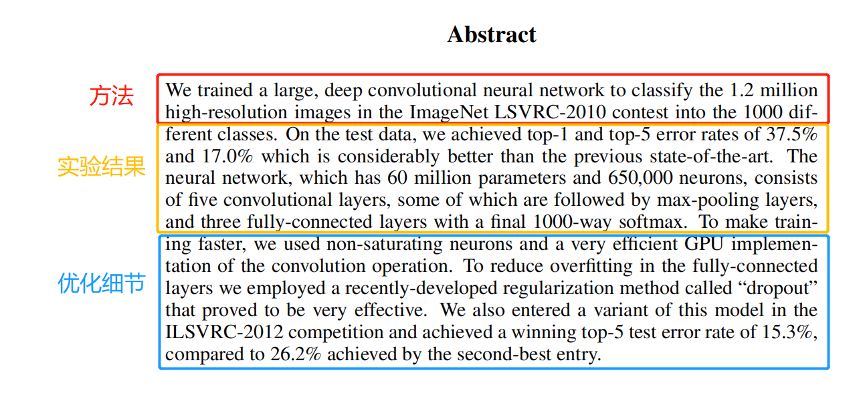
\includegraphics[width=\textwidth]{abstract}
	\caption{文章的摘要}
	\label{fig:abstract}
\end{figure}

在结构上,摘要采取了叙述文章采用的主要方法,即使用深度卷积神经网络进行图片分类,随后对实验结果进行了描述,最后通过叙述优化细节,来说明该文的方法是如何取得更优的效果。

这种摘要的结构是值得商榷的,一方面,对于大同行以及外行来说,这篇摘要并不完美,摘要并没有给出文章所面向的问题和研究意义,通过摘要无法对文章所面向的问题进行一个初步了解,如果将来论文需要面向大同行,建议将问题的背景进行补充;另一方面,对于小同行来说,这篇摘要已经能够充分反映研究中的必要信息,对于该文章所在领域来说,提高分类效率这一问题已经是此类与新模型相关的论文的共识性问题,关键在于新模型的结构以及效果如何,因此通过阅读这一摘要,即可清晰了解文章的工作及其意义。

在摘要内容的撰写方面,采用了简洁的纯文本进行叙述,语法上也没有较大的瑕疵,是值得肯定的。但摘要内容中出现了许多细节性数据,这一点是值得商榷的。摘要中给出了大量的细节性数据用于描述神经网络的模型架构、数据规模以及实验结果,显得不够简明扼要,如果将来论文需要面对大同行,建议将这些具体的实验数据略去,采用高度概括的词语进行叙述。但另一方面,对于小同行来说,根据这些细节性数据,已经可以较为全面的了解文章的工作以及效果。比如文章涉及领域面向大规模的图片分类问题,对于大同行来说,摘要中采用“大规模”这一概念描述即可,但对小同行来说,采用具体的数字规模说话,如该文中的“1.2 million”,更能直接反映文章模型的优势。此外,小同行还能够根据摘要中给出的一些模型关键参数的具体数值对文章设计的模型进行复现。

\section{引证}
对于引证部分,该文章均采用如图~\ref{fig:cited}所示的间接引用方式,引用的格式较为规范,参考文献的序号均紧跟在引证的主要内容后,且对于所引证的内容都通过简练的语言进行了转述,使之符合文章的表达情境。在文内的引用没有太大的问题,加之该文章作为深度学习领域的代表性论文,作者又是业界著名学者,其引证方式值得参考学习。
\begin{figure}[!htbp]
	\centering
	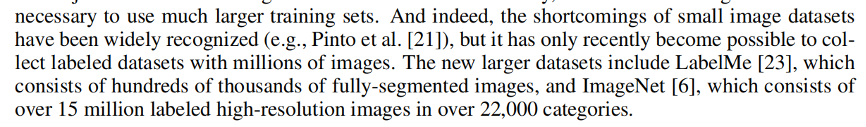
\includegraphics[width=\textwidth]{cited}
	\caption{文章中的引证示例}
	\label{fig:cited}
\end{figure}

对于引证的文献的范围来说,如图~\ref{fig:reference},可以看到,该文的引证范围较为全面,且参考文献的质量都较高。一方面,其覆盖了涉及领域早期的经典的奠基性文献,以及论文发表时期的最新研究成果;另一方面,其引用论文的质量较高,可以看到,引用文献许多来自于文章所属行业的顶级会议和顶级作者。此外,该文的引证文献均为公开文献,使得文章的引证是确实有据可查的。

\begin{figure}[!htbp]
	\centering
	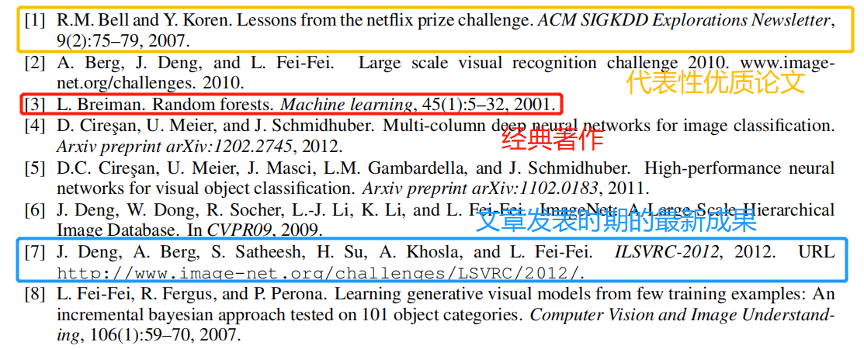
\includegraphics[width=\textwidth]{reference}
	\caption{文章的参考文献}
	\label{fig:reference}
\end{figure}

\chapter{引言部分的分析}\label{chap:introduction}

在Introduction部分,作者完成了五部分内容的说明,分别对应文章中的五段。

第一段,作者对图像分类这一领域简单的做了背景和现状的介绍,这一段内容相信不只是小同行,大同行都能轻松读懂。

第二段作者主要说明了如果在大规模数据集下使用前人方法会遇到的问题和挑战——任务的复杂性会非常高。

第三段作者根据上一段的问题和挑战提出了解决思路,Gpu和2D卷积相结合可以训练大型的CNN,且带标签数据集可以使模型不发生严重的过拟合。

第四段作者通过和前人方法的效果对比说明论文的贡献,在说明使用方法的同时,说明了文章的具体结构。

最后,在引言第五段,作者提出了可能存在的改进方法——只需要等更快的GPU和更大的数据集就可以得到更好的结果。

这五个部分内容同刘老师上课讲的完全一致,拥有了目的、核心任务、思路、贡献和文章结构5个要素。通过阅读引言,就能明白了作者想要解决什么样的问题,且该文作者只着重讲了一个问题的解决,也就是只有一个卖点——在大规模图片数据集上进行对象识别得到了比其他方法更好的结果,而这一点也是刘老师上课时强调的。

值得一提的是,该文提出问题的方式是“补”,也就是提出了Gap,在前人工作的基础上进行了改良,得到了比前人更好的结果。

纵观整个引言部分,作者精雕细琢,没有多写一句废话,没有介绍常识,也没有提及具体细节,对他人的工作也非常客观的做出了评价。


\chapter{方法、结果、讨论}\label{chap:res}
接下来,我们将对该文章使用的方法、得出的结果,以及该文章的讨论部分进行写作规范方面的分析。
\section{方法}
这篇文章在引言部分,就点出了当前三大主流研究方向——更大的数据集,具有更强大学习能力的模型,更好地处理过拟合的方法。而这三点也是一个神经模型实现的关键。方法部分,作者也是这样组织的。

首先,作者在第二部分数据集中,对模型采用的训练集和测试集进行了详细地介绍——ImageNet。由于本篇文章重点突出,在较大数据集上,如何训练出具有强大学习能力的模型,所以作者在数据集介绍过程中,突出强调ImageNet是一个超大型的高分辨率图像数据集。同时,作者说明了他们在训练过程中观测的重要指标,错误率(top-1和top-5)。另外,作者也描述了他们对数据的预处理,为模型效果复现提供了必要的基础。

方法第三部分便是模型的框架。作者开篇介绍网络共8层——5个卷积层和3个全连接层,这好比是一个具体模型的骨架。在3.1至3.4节中,作者针对模型架构中新颖的特点,按照重要程度,一一进行了介绍。这些好比是依附在骨架上的血肉,而正是这些与前人不同的特点,使得Alexnet2012成为了当时图像分类最好的模型。其中包括非线性ReLU方法,更是成为了今后解决梯度消失问题经典方法。

方法的第四部分则是针对处理过拟合问题的方法,结构与第三部分相似,分条列出两种主要方法——数据增强和Dorpout。
\section{结果}

文章的结果采用报告实验型结果,如表~\ref{tab:tbl1}、表~\ref{tab:tbl2}所示。文章给出了Alexnet模型与其他人(表中的斜体部分)效果最好的模型的Top-1和Top-5错误率,清晰直观地显现出Alexnet模型在图像分类上的优越性。同时,在定量描述之外,作者还对结果进行了定性评估,分析模型在特定数据集上的效果,图文并茂,直观明了。

\section{讨论}
作者在讨论部分对全文进行了总结,在强调模型在具有挑战性的大型数据集上取得破纪录的结果同时,点出了模型的不足之处——模型可以更大,训练时间可以更长。同时提出了新的问题,给阅读者提供了未来新的研究方向——希望在视频序列中使用非常大且深的卷积网络。
\chapter{图表分析}\label{chap:figtbl}
文章中图表的类型比较丰富,可以粗略分为视觉型插图和文字型插图,以下从宏观和微观两个角度来分析该文章的图表。

\section{从宏观角度分析}
从宏观的角度来看,我们可以从以下4个方面进行分析:
\begin{enumerate}
\item
插图的数量,文章共有9页,共有9张插图,平均每页一张插图,让读者阅读起来不会产生视觉疲劳
\item
插图的类型,文中视觉型插图(如图~\ref{fig:visualp})有4张,文字型插图(公式和表格,如图~\ref{fig:textp})共5张,类型配比接近1:1,类型均衡
\begin{figure}[!htbp]
    \centering
    \begin{subfigure}[b]{0.35\textwidth}
      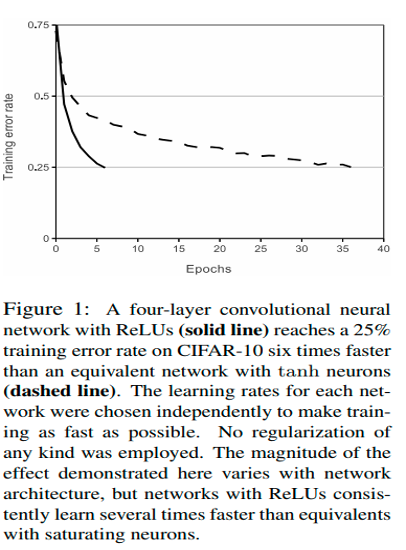
\includegraphics[width=\textwidth]{visualp1}
      \caption{}
      \label{fig:oaspl_a}
    \end{subfigure}%
    ~% add desired spacing
    \begin{subfigure}[b]{0.35\textwidth}
      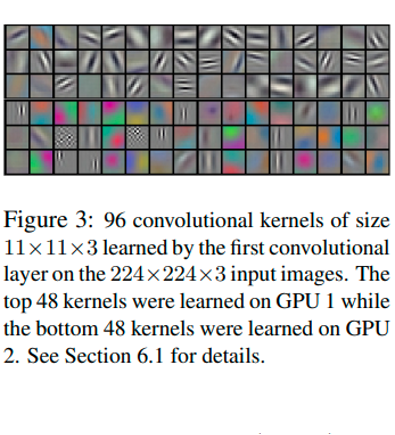
\includegraphics[width=\textwidth]{visualp2}
      \caption{}
      \label{fig:oaspl_b}
    \end{subfigure}
    \\% line break
    \begin{subfigure}[b]{0.35\textwidth}
      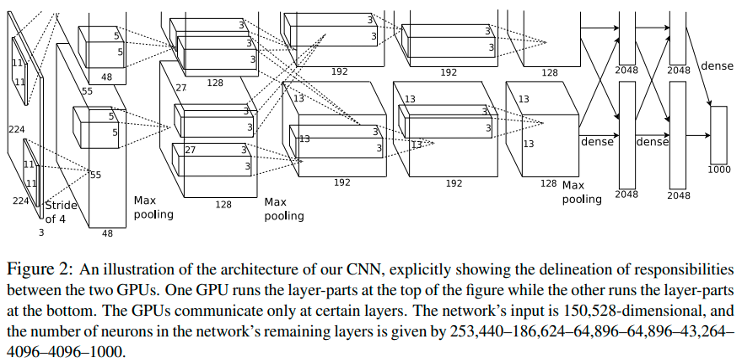
\includegraphics[width=\textwidth]{visualp3}
      \caption{}
      \label{fig:oaspl_c}
    \end{subfigure}%
    ~% add desired spacing
    \begin{subfigure}[b]{0.35\textwidth}
      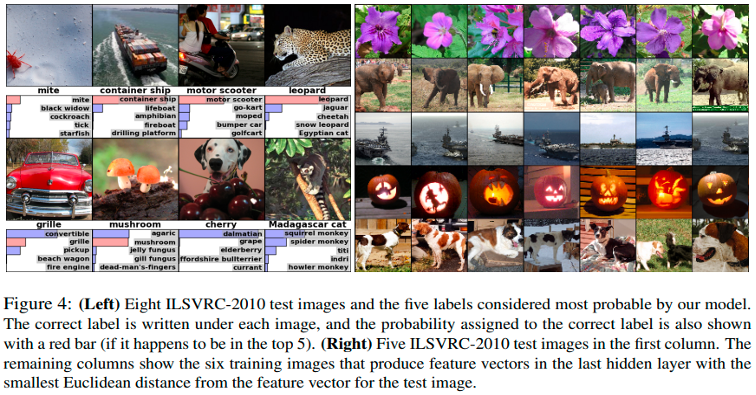
\includegraphics[width=\textwidth]{visualp4}
      \caption{}
      \label{fig:oaspl_d}
    \end{subfigure}
    \caption{视觉型插图}
    \label{fig:visualp}
\end{figure}

\begin{figure}[!htbp]
    \centering
    \begin{subfigure}[b]{0.35\textwidth}
      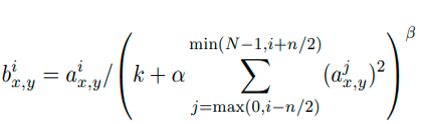
\includegraphics[width=\textwidth]{textp1}
      \caption{}
      \label{fig:oaspl_a}
    \end{subfigure}%
    ~% add desired spacing
    \begin{subfigure}[b]{0.35\textwidth}
      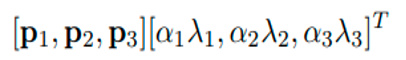
\includegraphics[width=\textwidth]{textp2}
      \caption{}
      \label{fig:oaspl_b}
    \end{subfigure}
    \\% line break
    \begin{subfigure}[b]{0.35\textwidth}
      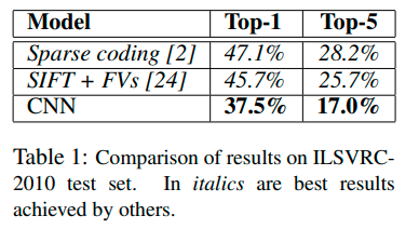
\includegraphics[width=\textwidth]{textp4}
      \caption{}
      \label{fig:oaspl_c}
    \end{subfigure}%
    ~% add desired spacing
    \begin{subfigure}[b]{0.35\textwidth}
      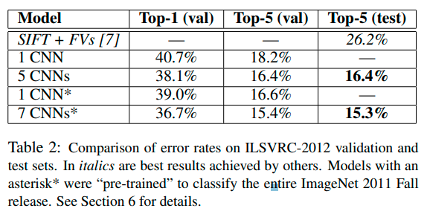
\includegraphics[width=\textwidth]{textp5}
      \caption{}
      \label{fig:oaspl_d}
    \end{subfigure}
    ~% add desired spacing
    \begin{subfigure}[b]{0.35\textwidth}
      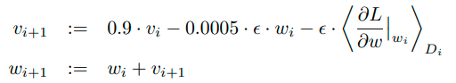
\includegraphics[width=\textwidth]{textp3}
      \caption{}
      \label{fig:oaspl_d}
    \end{subfigure}
    \caption{文本型插图。(a) 位于3.3节 ,(b) 位于4.1节,(c) 位于第6节,(d) 位于第6节,(e)位于第5节。}
    \label{fig:textp}
\end{figure}

\item
插图在文中的位置分布,文章分为7部分,其中第3-6节是主体部分,在3.1节、3.5节、第5节、6.1节中各有一张视觉型插图,在3.3节、4.1节、第5节各有一个公式,第6节有两张表格。不难发现:图表在各节的分布也很均衡,同一小节最多不会多于2张插图,且除第6节外,每一节插图的类型都不一样,同时也没有图表的堆叠,给读者带来了良好的视觉体验,且能实时结合图表,有助于对文章内容的理解把握。
\item
内容和插图的排版,文中的插图和文字内容部分大部分很合理,除了第6节中的两张表格,如图~\ref{fig:improper}所示。

其中表格的位置对文字表述部分造成了冲击,使得一个单词跨两行的现象增多,让排版变得有些混乱,一定程度上影响了读者的阅读体验。我们认为,让文字环绕在表格上下,同时将表格的标题行数减少(同时增加每行容纳的词数),带来的视觉效果更好。
\end{enumerate}
% 1.	插图的数量,文章共有9页,共有9张插图,平均每页一张插图,让读者阅读起来不会产生视觉疲劳
% 2.	插图的类型,文中视觉型插图有4张,文字型插图(公式和表格)共5张,类型配比接近1:1,类型均衡 
% 3.	插图在文中的位置分布,文章分为7部分,其中第3-6节是主体部分,在3.1节、3.5节、第5节、6.1节中各有一张视觉型插图,在3.3节、4.1节、第5节各有一个公式,第6节有两张表格。不难发现:图表在各节的分布也很均衡,同一小节最多不会多于2张插图,且除第6节外,每一节插图的类型都不一样,同时也没有图表的堆叠,给读者带来了良好的视觉体验,且能实时结合图表,有助于对文章内容的理解把握。 
% 4.	内容和插图的排版,文中的插图和文字内容部分大部分很合理,除了第6节中的两张表格,如图~\ref{fig:improper}所示:
\begin{figure}[!htbp]
	\centering
	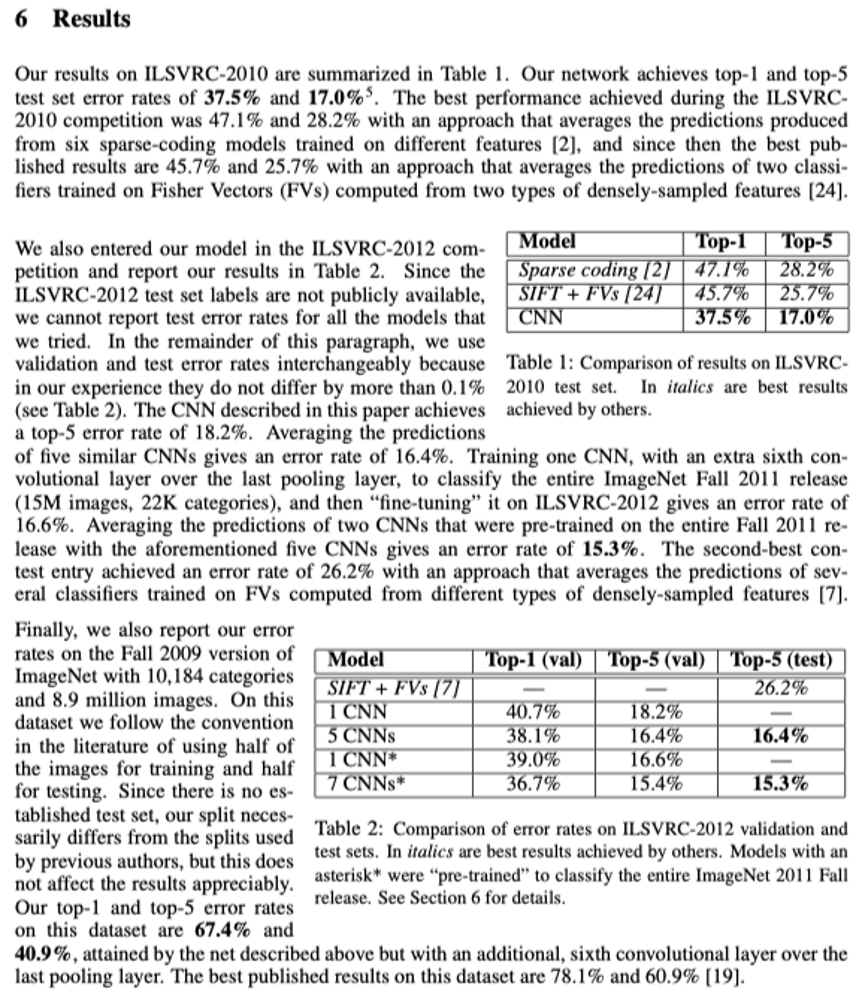
\includegraphics[width=\textwidth]{improper}
	\caption{不合理的表格排版}
	\label{fig:improper}
\end{figure}

\section{从微观角度分析}
从微观的角度来看,可以从以下2个方面进行分析。
\begin{enumerate}
\item 视觉型插图,视觉型插图包含了图表、图示、图片,每张插图的标题都清楚的对插图进行了说明,做到了自明,同时图标、图示结构简洁清晰,图片的组合清晰美观,不得不说,该文的视觉型插图做的很棒,让读者能够更加直观的理解文章提出的CNN网络以及它的功能;
\item 文本型插图,其中包含了公式和表格,公式并没有大量使用,只是在论述过程中恰如其分的用来准确的表达概念,且所使用的公式形式简单,对大多数读者而言,增强了可读性,更易于理解;表格做到了自明,所表达的内容也不冗余,通过与其他模型的量化对比,让读者清晰直观的掌握到CNN网络的性能,但表格还有改进的空间,例如改为如表~\ref{tab:tbl1}、表~\ref{tab:tbl2}形式:

\end{enumerate}
% Table generated by Excel2LaTeX from sheet 'Sheet1'
\begin{table}[!htbp]
  \renewcommand\arraystretch{0.8}
  \centering
  \caption{修改后的Table 1}
    \begin{tabular}{p{10.915em}rr}
    \toprule
    \textbf{Model} & \multicolumn{1}{c}{\textbf{Top-1}} & \multicolumn{1}{c}{\textbf{Top-5}} \\
    \midrule
    \textit{Sparse coding [2]} & \multicolumn{1}{c}{\textit{47.10\%}} & \multicolumn{1}{c}{\textit{28.20\%}} \\
    \textit{SIFT+FVs [24]} & \multicolumn{1}{c}{\textit{45.70\%}} & \multicolumn{1}{c}{\textit{25.70\%}} \\
    \textbf{CNN} & \multicolumn{1}{c}{\textbf{37.50\%}} & \multicolumn{1}{c}{\textbf{17.00\%}} \\
    \midrule
    \multicolumn{3}{p{22.415em}}{Table 1: Comparison of results on ILSVRC2010 test set. In italics are best results achieved by others} \\
    \end{tabular}%
  \label{tab:tbl1}%
\end{table}%

% Table generated by Excel2LaTeX from sheet 'Sheet1'
\begin{table}[!htbp]
  \renewcommand\arraystretch{0.8}
  \centering
  \caption{修改后的Table 2}
    \begin{tabular}{p{8.215em}lp{8.215em}rp{8.215em}cp{8.215em}c}
    \toprule
    \textbf{Model} & \multicolumn{1}{c}{\textbf{Top-1(val)}} & \multicolumn{1}{c}{\textbf{Top-5(val)}} & \multicolumn{1}{c}{\textbf{Top-5(test)}} \\
    \midrule
    \textit{SIFT+FVs[7]} & \multicolumn{1}{p{8.215em}<{\centering}}{—} & \multicolumn{1}{c}{—} & \multicolumn{1}{c}{\textit{28.20\%}} \\
    1CNN  & \multicolumn{1}{c}{40.70\%} & \multicolumn{1}{c}{18.20\%} & \multicolumn{1}{c}{—} \\
    5CNNs & \multicolumn{1}{c}{38.10\%} & \multicolumn{1}{c}{16.40\%} & \multicolumn{1}{c}{\textbf{16.40\%}} \\
    1CNN* & \multicolumn{1}{c}{39.00\%} & \multicolumn{1}{c}{16.60\%} & \multicolumn{1}{c}{—} \\
    7CNNs* & \multicolumn{1}{c}{36.70\%} & \multicolumn{1}{c}{15.40\%} & \multicolumn{1}{c}{\textbf{15.30\%}} \\
    \midrule
    \multicolumn{4}{p{32.92em}}{Table 2: Comparison of error on ILSVRC-2012 validation and test sets. In italics are best results achieved by others. Models with an asterisk* were “pre-trained” to classify the entire ImageNet 2011 Fall release. See Section 6 for details.  } \\
    \end{tabular}%
  \label{tab:tbl2}%
\end{table}%


\chapter{小结}\label{chap:conclude}
本报告对文章《ImageNet Classification with Deep Convolutional Neural Networks》进行了写作规范的研究。经过分析,我们认为该文章在写作规范的角度上是非常不错的,但是仍然有一些值得商榷、值得改进的小细节。

首先,我们认为该文章的摘要部分可以进一步改进,使得大同行也能通过文章的摘要更加理解该文章的价值。

其次,我们认为该文章的图表中,有两个表格的格式、排版不是很合理,所以我们在报告的正文部分给出了更加合理的表格格式。

%---------------------------------------------------------------------------%
% main content
%-
%-> Appendix
%-
\cleardoublepage%
% \appendix% initialize the environment
% \input{Tex/Appendix}% appendix content
%-
%-> Backmatter: bibliography, glossary, index
%-
% \backmatter% initialize the environment
% \intotoc*{\cleardoublepage}{\bibname}% add link to toc
% \artxifstreq{\artxbib}{bibtex}{% enable bibtex
%     \bibliography{Biblio/ref}% bibliography
% }{%
%     \printbibliography% bibliography
% }
%\input{Tex/Backmatter}% other information
\end{document}
%---------------------------------------------------------------------------%

